\documentclass[10pt,a4paper]{article}
\usepackage[utf8]{inputenc}
\usepackage[francais]{babel}
\usepackage[T1]{fontenc}
\usepackage{charter}
\usepackage[top=2cm, bottom=2cm, inner=2cm, outer=2cm]{geometry}
\usepackage{amsmath}
\usepackage{amsfonts}
\usepackage{amssymb}
\usepackage{graphicx}
\usepackage{lipsum}
\usepackage{authblk}
\renewcommand*{\Authand}{ et }
\AddThinSpaceBeforeFootnotes
\FrenchFootnotes

\title{NATURE : Figures avec \LaTeX \ \& Python}
\author[1]{Aurélien Carré}
\author[1]{Pierre Nagorny}
\affil[1]{Laboratoire pour le Prix Nobel de la Mécatronique 2017}
\date{10 janvier 2017}
\begin{document}
\maketitle

\begin{figure}[h]
\begin{center}
\includegraphics[width = .5\textwidth]{fete-science.jpg}
\caption{Le logo de la fête de la science !}
\end{center}
\end{figure}

\begin{abstract}
    Le deeplearning permet aujourd'hui d'écrire une thèse mais également un article. Ces avancés ouvrent de larges champs de recherche avec nombreuses publications à la clé.
\end{abstract}

\section{Introduction}
Le deeplearning permet aujourd'hui d'écrire une thèse. Cette article est également écrit en deeplearning.
L'apprentissage est réaliser en 12 heures sur l'ensemble des articles publiés dans Nature depuis 1903.
Le deeplearning permet de produire des publication acadméiques dans de grandes revues en payant simplement l'abonnement à la revue (25 000\$) et une machine louée dans un cloud. L'indice h de l'auteur possédant ce pouvoir est alors augmenté.



\section{L'oscillateur du Temps de la Vie}
\begin{figure}[h]
\begin{center}
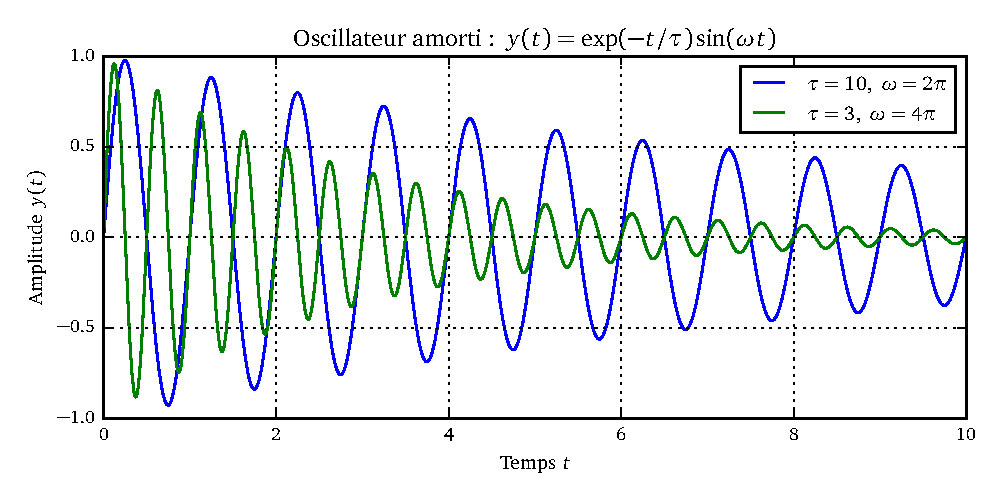
\includegraphics{Oscillateur}
\end{center}
\caption{Un oscillateur de la Vie du Temps en activité}
\end{figure}

\section{Lorem ipsum dolor}

\lipsum[1-13]

\section{Comment faire une bonne purée}
\begin{figure}[h]
\begin{center}
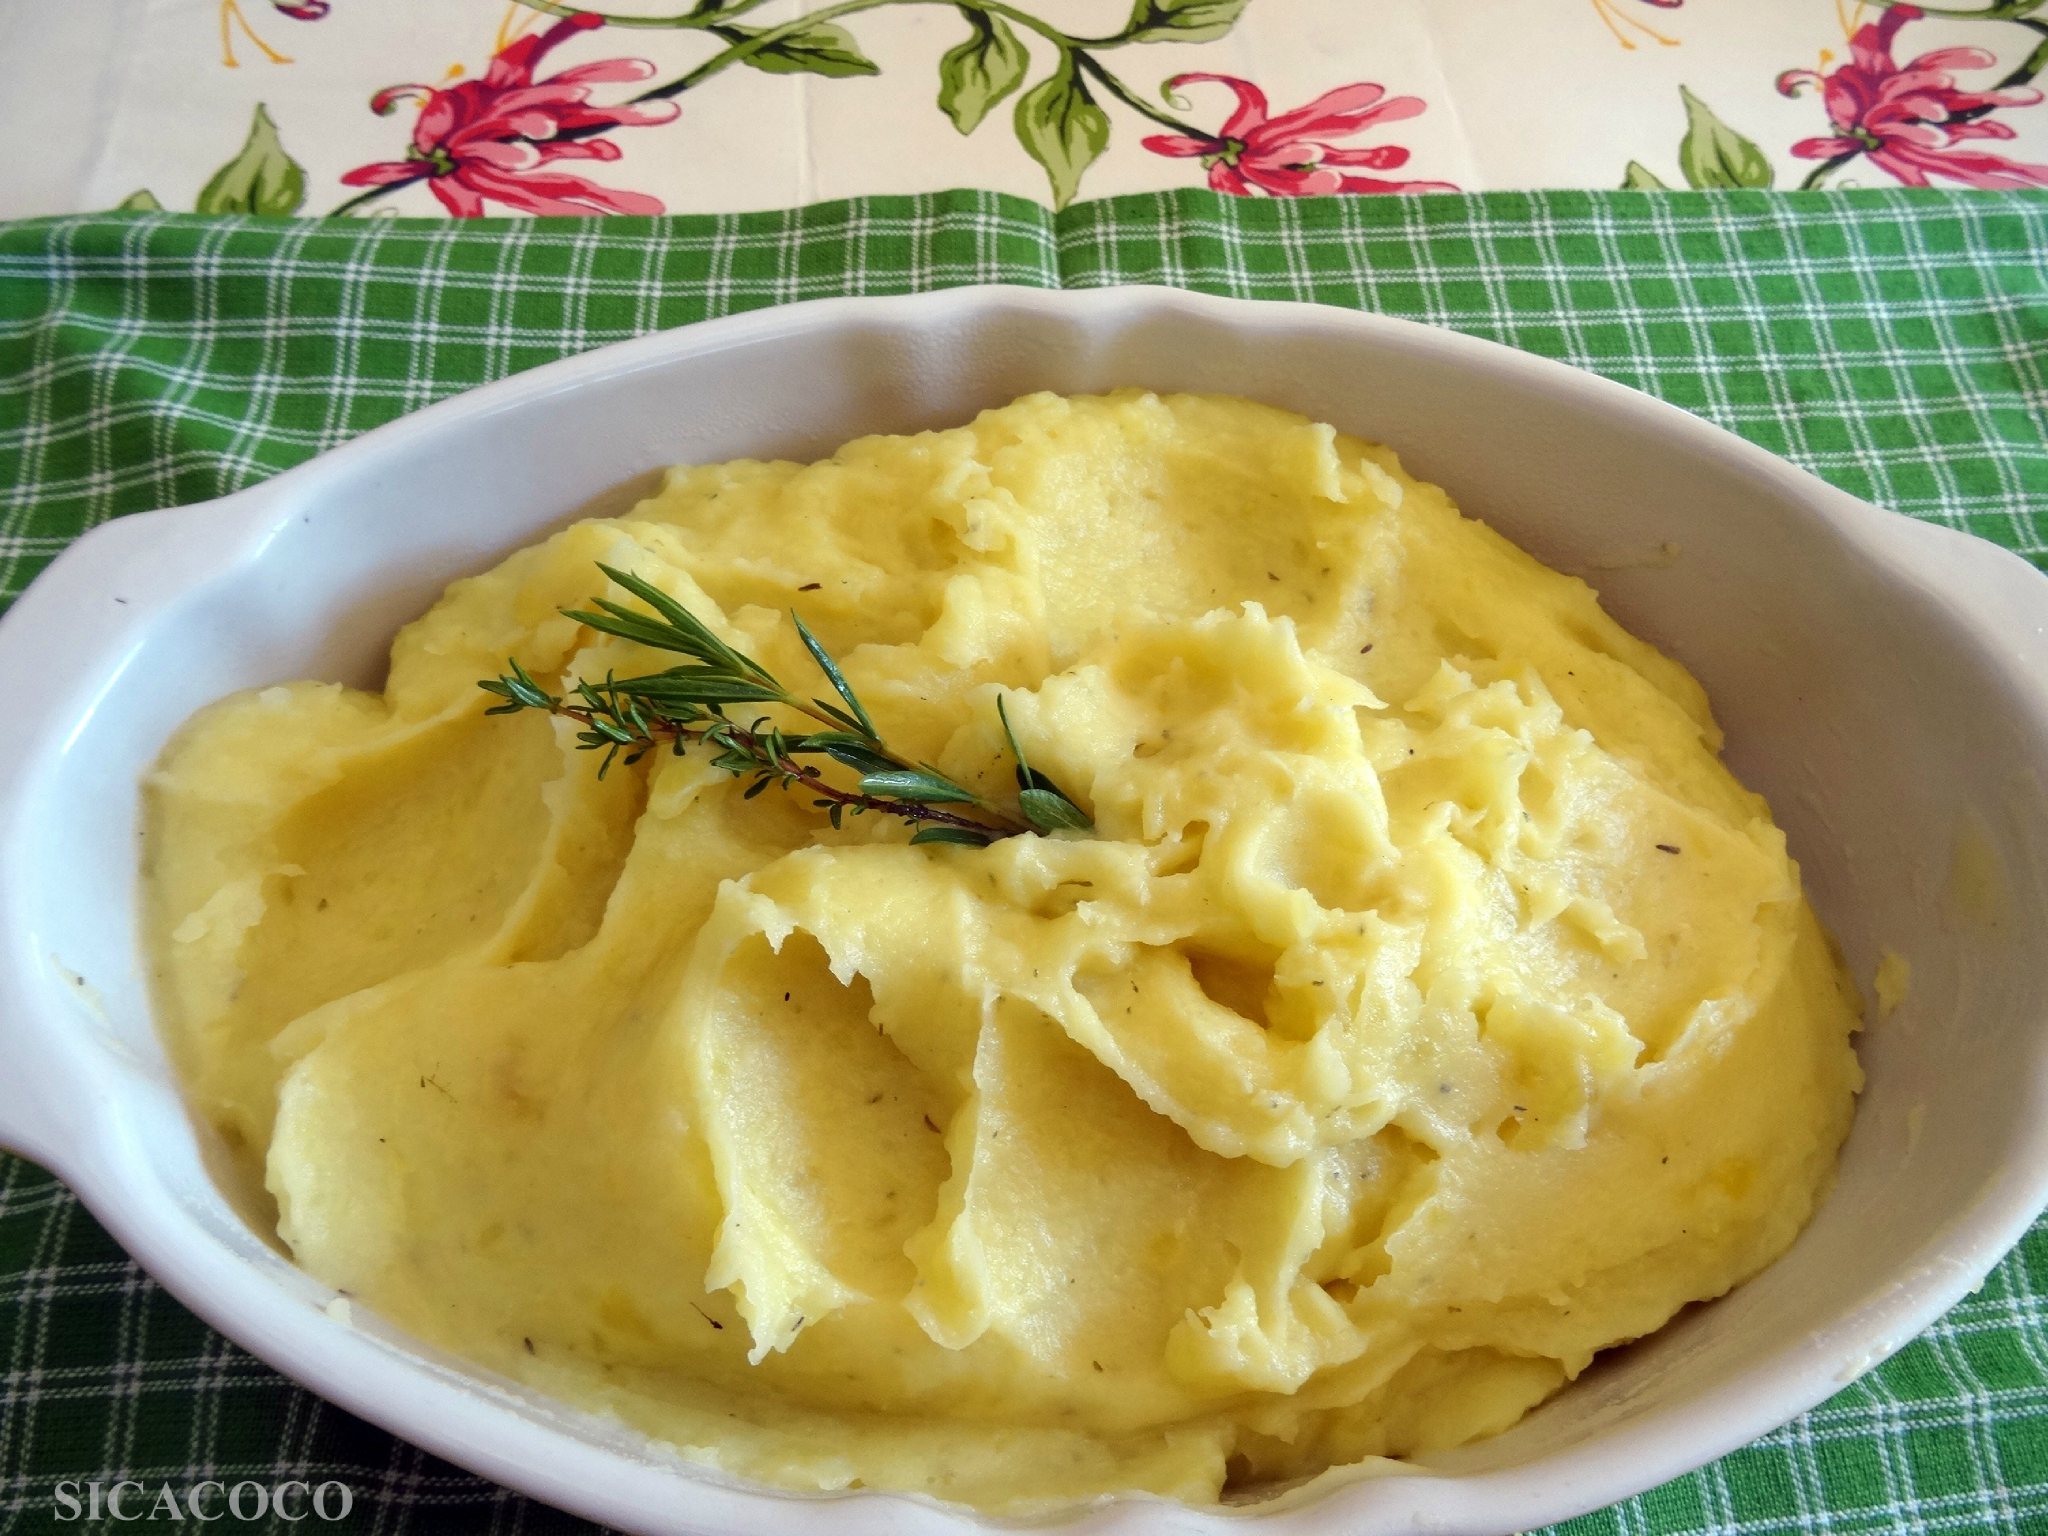
\includegraphics[width = .8\textwidth]{96234589_o}
\end{center}
\caption{Une purée réussie}
\label{fig:puree}
\end{figure}


\begin{center}
Salut, \newline
J'aimerais savoir comment faire une bonne purée \newline
Je sais déjà faire la ratatouille, les endives au jambon, le gratin \newline
Et plein d'autres plats qui n'ont rien à voir avec une bonne purée. \newline
Quel est votre secret ? \newline
Le lait ? \newline
Le beurre ? \newline
La crème ? \newline \newline
Quel est votre secret ? \newline \newline
S'il vous plait aidez-moi \newline \newline
Quel est votre secret ? \newline
Pour faire une bonne purée ce qui est pas mal quand on cuit les pommes de terre \newline
C'est de mettre du laurier et du thym pour parfumer en amont \newline
Après tu peux ajouter n'importe quel épice \newline
Tu peux mettre du safran, du curcuma, du gingembre \newline
Ou une gousse d'ail une fois que les patates sont pétries \newline
Et si la purée a cramé \newline
Recouvre-la avec un chiffon mouilé \newline
Et fais couler du sel dessus \newline
Pour absorber les senteurs de brûlé \newline
\newline
Excuse moi mais c'est pas ça que j'avais demandé \newline
Le problème avec ma purée c'est qu'elle n'est pas onctueuse \newline
Peux-tu m'expliquer, comment obtenir une texture parfaite ? \newline
La purée onctueuse ce qu'il faut déjà \newline
C'est pas trop la mélanger ou l'écraser \newline
Puisque comme dans la purée il y a du gluten ça va devenir très élastique \newline
L’utilisation du presse-purée à levier permet d’obtenir une purée plus fine et légère \newline
Tout est dans la texture \newline
Car la purée trop collante est vraiment très décevante \newline
Pense à ça avant de cuisiner et tu réussiras une bonne purée \newline
Tu verras, c'est plus facile que ça en a l'air \newline
Et surtout après ça tu ne voudras plus d'une autre purée \newline
J'ai 4 hommes à la maison et ils se régalent tous \newline
Il n'en reste jamais ! \newline
\end{center}

La figure \ref{fig:puree} (page \pageref{fig:puree}) est issue de l'Internet.



\end{document}
